\documentclass[12pt,a4paper]{article}
\usepackage{appendix}
\usepackage[utf8]{inputenc}
\usepackage[french]{babel}
\usepackage[T1]{fontenc}
\usepackage{amsmath}
\usepackage{amsfonts}
\usepackage{amssymb}
\usepackage{graphicx}
\usepackage[left=2cm,right=2cm,top=2cm,bottom=2cm]{geometry}
\usepackage{ccaption}
\author{Javaid Mohammad-Habib, Carbonneau Danaël}

\usepackage[Glenn]{fncychap}

\usepackage{fancybox}

\usepackage{multicol}
\usepackage[hidelinks]{hyperref}

\usepackage{xcolor}
\usepackage{tcolorbox}
\usepackage{listings}


	
	
\definecolor{darkWhite}{rgb}{0.94,0.94,0.94}
 
\lstset{
  aboveskip=3mm,
  belowskip=-2mm,
  backgroundcolor=\color{darkWhite},
  basicstyle=\footnotesize,
  breakatwhitespace=false,
  breaklines=true,
  captionpos=b,
  commentstyle=\color{green},
  extendedchars=true,
  framexleftmargin=16pt,
  framextopmargin=3pt,
  framexbottommargin=6pt,
  frame=tb,
  keepspaces=true,
  keywordstyle=\color{blue},
  otherkeywords={module},
  language=caml,
  morekeywords={*,...},
  numbers=left,
  numbersep=10pt,
  numberstyle=\tiny\color{black},
  rulecolor=\color{black},
  showspaces=false,
  showstringspaces=false,
  showtabs=false,
  stepnumber=1,
  stringstyle=\color{gray},
  tabsize=4,
  title=\lstname,
}	
	
	
	
	
\usepackage{enumitem}
\usepackage{pifont}
\setitemize[1]{font=\bfseries, label= \color{teal} \ding{227}  }
\setitemize[0]{font=\bfseries, label= \color{olive} \ding{216}  }


\begin{document}


\begin{titlepage}
\newcommand{\HRule}{\rule{\linewidth}{0.5mm}}



\center 
\bigskip
\textsc{\LARGE
Sorbonne Université
}
 \\[4cm]
 \HRule \\[0.4cm]
{ \huge \bfseries Devoir de Programmation \\[0.15cm] }
\textbf{UE d'Ouverture}
\HRule \\[0.5cm]

Danaël CARBONNEAU (28709878), Javaid Mohammad-Habib (21307723) \\[2cm]

\begin{huge}
Diagrammes de décision binaires (\textit{ZDD}).
\end{huge}

\vfill

\textit{Enseignants : Antoine Genitrini, Emmanuel Chailloux}

Master STL, Semestre 1, septembre - janvier 2023 - 2024 \\ [1cm]

\end{titlepage}



\tableofcontents



\newpage

\section{Échauffement}

Le code associé à cette partie se trouve dans le fichier \textit{echauffement.ml}. 

Nous représenterons dans la suite du projet les entiers précis par ce type : \texttt{type entier\_precis = int64 list;;}. Nous avons également écrit pour les manipuler une primitive permettant l'ajout en fin, une permettant de récupérer la tête, et une permettant de récupérer sa suite.

Par la suite, nous avons pu écrire les fonction nous permettant de manipuler les grands entier sous plusieurs représentations (listes d'entiers 64 bits, listes de booléens). Grâce aux fonctions \texttt{Int64.unsigned\_rem} \texttt{Int64.shitf\_right\_logical}, et \texttt{Int64.shift\_left}, on traite bien notre entier comme s'il n'était pas signé, donc en utilisant ses 64 bits.

Concernant la génération aléatoire, depuis la version \href{4.14}{https://ocaml.org/releases/4.14.0}, le module Random implémente une fonction \texttt{Random.bits64()} qui nous retourne 64 bits aléatoires représentés sur un entier 64 bits. Lorsqu'on teste \texttt{GenAlea}, on voit alors bien des nombres négatifs apparaître dans la décomposition (c'est à dire des nombres ayant leur bit de poids fort à 1, ce qui correspond à ce qu'on veut pour traiter les entiers 64 bits de la liste comme des bitmaps). Il est donc nécessaire d'avoir cette version d'installée.
%TODO : annexe howto installer ocaml 4.14.1


\section{Arbres de Décision}
Le code associé à cette partie se trouve dans le fichier \textit{Arbre\_decision.ml}.

La structure est faite à l'aide d'un type Somme (et d'un alias de type pour la profondeur) :

\medskip

\begin{lstlisting}
type profondeur = int
type arbre_decision = 
	| Feuille of boolean 
	| Noeud of profondeur* arbre_decision * arbre_decision.
\end{lstlisting}
\medskip


\section{Compression de l’arbre de décision et ZDD}

Le code associé à cette partie se trouve dans les fichiers \textit{deja\_vus.ml}, \textit{compression.ml}, et \textit{dot.ml}.

\subsection{Choix d'implémentation : l'utilisation de foncteurs}

L'algorithme de compression utilise une structure permettant de conserver une trace des grands entiers déjà vus. Étant donné que nous serons amenés à utiliser cette algorithme avec deux structures (une liste dans cette partie, une arborescence dans la suivante), nous avons décidé d'utiliser le mécanisme de \textbf{foncteurs} offertes par le langage OCaml.

En effet, du point de vue de l'algorithme, il nous faut une structure qui nous rend trois services : 

\begin{itemize}
\item créer une structure vide
\item insérer un couple (grand entier, arbre de décision) dans la structure
\item déterminer si un grand entier est dans la structure (auquel cas, retourner l'arbre de décision associé, rien sinon).
\end{itemize}

On va donc définir un type de modules correspondant à cette interface : il s'agit du module \texttt{SetDejaVus}, dont la signature est donnée dans \textit{deja\_vus.ml}.

De là, on veut pouvoir utiliser n'importe quelle structure pour laquelle seraient définis ces trois services dans notre algorithme. Pour cela, on va écrire, dans \textit{compression.ml} un foncteur \texttt{AlgoCompression}, c'est à dire un module paramétré par le type de modules \texttt{SetDejaVus}. À l'intérieur de ce foncteur, on peut désormais écrire notre fonction de compression, qui utilise le module passé en paramètres pour avoir :
\begin{itemize}
\item Le type de la structure utilisée
\item Les opérations, qui sont nécessaires à l'algorithme, dont l'implémentation va dépendre de la structure
\end{itemize}


On arrive ainsi à factoriser notre code et séparer le déroulement de l'algorithme de la gestion sous-jacente, de notre ensemble d'arbres déjà vus.






\subsection{Manipulation des arbres de compression}

Dans l'algorithme de compression, nous voulons remplacer, lorsqu'une règle de compression est appliquée, le noeud courant N par un autre noeud vis à vis de son père. Étant donné que notre fonction reconstruit l'arbre compressé en fonction des appels récursifs, il nous suffit pour cela de retourner le bon nœud remplaçant le nœud N par celui qui lui correspond dans notre arbre compressé.

La représentation des valeurs, et notamment des types sommes, nous permet de ne pas avoir besoin d'utiliser de références : les valeurs en OCaml sont soit des entiers , soit des pointeurs vers un bloc sur le tas. Lorsqu'on ajoute un noeud en tête de notre ensemble de (grand entier, noeud) déjà visités, on créé sur le tas un bloc contenant un pointeur vers notre noeud, et un pointeur vers la suite de la liste. Lorsqu'on le récupère ailleurs dans le code, on ne récupère alors pas de copie mais bien un pointeur vers le nœud souhaité. 


\subsection{La fonction compressionParListe}

\subsubsection{Le module \texttt{SetList}}

La première approche pour représenter notre ensemble de couples \texttt{(grand\_entier, arbre\_decision)} est de le faire par une liste. Il nous suffit pour ça d'écrire un module \texttt{SetList}, dont la signature est décrite par \texttt{SetDejaVu}. Sa structure  comporte : 


\begin{itemize}
\item Un type ens défini comme une liste de couples \texttt{(grand\_entier, arbre\_decision)}
\item La valeur empty, définie comme étant une liste vide
\item Une fonction d'insertion, qui se fait par un simple ajout en tête dans la liste.
\item Une fonction de recherche, qui se fait en parcourant la liste en comparant les grands entiers présents avec celui passé en paramètres, et en rendant un \texttt{arbre\_decision option} (\texttt{Some(arbre)} s'il est présent dans la liste, \texttt{None} sinon).

\end{itemize}

\subsubsection{Définir la fonction grâce aux modules et au foncteur}

Maintenant que nous avons un module décrivant une manière de gérer ces ensembles, nous pouvons instancier le foncteur AlgoCompression en lui passant en paramètres notre module \texttt{SetList} avec \texttt{module FL = AlgoCompression(SetList)}

On peut alors définir la fonction compressionParListe avec ce foncteur : \texttt{let compressionParListe = FL.compression}.


\subsection{Faire des graphiques avec le langage dot}

Dans le fichier \textit{dot.ml}, nous avons écrit deux fonctions : une qui parcourt l'arbre de décision pour écrire dans un fichier ce qu'il faut pour chaque nœud, et une qui s'occupe de formater comme souhaité chaque noeud.

\subsubsection{Formatage en dot}

Dot nous permet de faire des graphes en décrivant les arrêtes, et potentiellement les nœuds, en les écrivant lignes après lignes. Il nous faut donc, pour transcrire facilement notre graphe, un identifiant unique par nœud (qui ne sera pas affiché, grâce aux labels). On peut ensuite, pour chaque nœud interne du graphe, écrire dans notre fichier la mise en forme correspondante : 


\begin{lstlisting}
Noeud(profondeur, fils_gauche, fils_droit)  -> 
	idNoeud [label = profondeur];
	idNoeud -> idFils_gauche [style=dotted]; 
 	idNoeud -> idFils_droit [style=dotted];

| Feuille(boolean) ->  idN [label = boolean];
\end{lstlisting}

\subsubsection{Des identifiants uniques... avec un peut de magie}
Afin d'avoir un \textbf{idN unique}, nous avons choisi d'utiliser la fonction \texttt{Obj.magic}. Il s'agit d'une fonction (\textit{peu recommandée}) de la librairie standard OCaml : elle force un cast de type sur l'objet qu'elle manipule (soit un entier, soit un bloc, donc un pointeurs vers le tas), qui est dans tous les cas codé sur un entier (soit de taille 32bits, doit de taille 64), et retourne sa valeur "réelle" (au runtime). 

Étant donné que nous appliquons cette fonctions à des arbres de décision, c'est à dire un type somme, c'est une manière de récupérer l'adresse de chaque block. Il s'agit donc d'un nombre \textbf{unique} à chaque nœud dans notre arbre, ce qui en fait un candidat parfait pour notre identifiant\footnote{Le système d'identifiant par pointeur nous permet également de vérifier que la compression s'est aussi faite en mémoire.}.


\subsubsection{Résultats}

Nous avons alors pu obtenir un affichage graphique de l'arbre de l'énoncé avant (\ref{fig1}) et après compression (\ref{fig2}). 


\begin{figure}[hbtp]
\centering
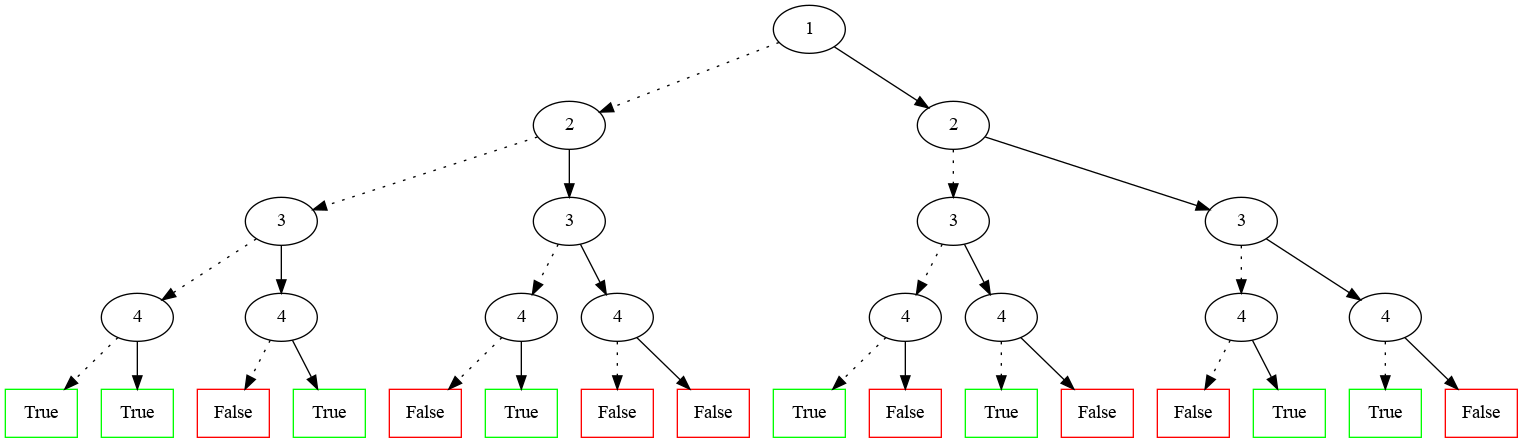
\includegraphics[scale=0.3]{../Images/arbre_non_compresse.png} 
\caption{Arbre de décision issu de la table de vérité de taille 16 construite sur [25899]}
\label{fig1}
\end{figure}


\newpage
\begin{figure}[hbtp]
\centering
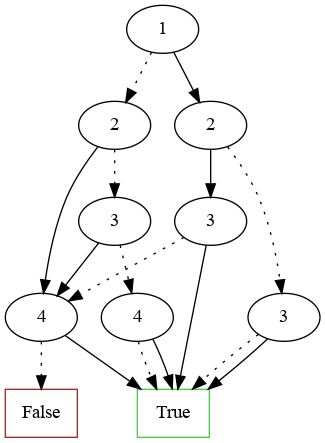
\includegraphics[scale=0.5]{../Images/arbre_compresse_par_liste.png}
\caption{ZDD construit sur le grand entier [25899],\\ compressé avec CompressionParListe}
\label{fig2}
\end{figure}

L'algorithme de compression que nous avons écrit nous semble alors fonctionner conformément aux attentes.

\section{Compression avec historique stocké dans une structure arborescente}

Le code correspondant à la structure arborescente se trouve dans le module \texttt{SetTree}, présent dans le fichier \textit{deja\_vus.ml}. La définition de la fonction de compression dans \textit{compression.ml}.

\subsection{La fonction compressionParArbre}

\subsubsection{Le module \texttt{SetTree}}
Le module \texttt{SetTree} répond à la signature décrite par \texttt{SetDejaVu}. Sa structure comporte : 


\begin{itemize}
\item Un type ens défini comme un arbre dont les feuilles sont vides et les nœuds sont des \texttt{arbre\_decision option}, c'est-à-dire qu'il peut soit y avoir un arbre de décision sur le nœud, soit rien.

\item La valeur empty, définie comme étant une feuille.

\item Une fonction d'insertion, qui se fait en parcourant les bits du grand entier du couple à insérer en allant dans le sous arbre gauche si le bit est à 0, à droite si le bit est à 1. Lorsqu'on a fini de parcourir les bits, on insère le pointeur dans le nœud courant\footnote{Dans le cas, qui n'est pas interdit par notre structure, mais qui ne devrait pas arriver vue la manière dont on se sert de ces arborescences, où on insère un couple dont le grand entier est déjà dans l'arborescence, on remplace l'ancienne valeur du pointeur par la nouvelle.}. 

\item Une fonction de recherche, qui se fait en parcourant les bits du grand entier du couple en suivant le même aiguillage. Lorsqu'on a fini de regarder les bits du grand entier, on retourne le \texttt{arbre\_decision option} correspondant (\texttt{None} s'il n'y a pas le pointeur).
\end{itemize} 


\subsubsection{Définir la fonction \texttt{compressionParArbre}}

Maintenant que nous avons un module décrivant une manière de gérer ces ensembles avec des arbres, nous pouvons instancier le foncteur \texttt{AlgoCompression} en lui passant en paramètres notre module \texttt{SeTree}, on peut alors définir la fonction \texttt{compressionParArbre} avec ce foncteur : 

\bigskip
\begin{lstlisting}
module FT = AlgoCompression(SetTree)
let compressionParArbre = FT.compression

\end{lstlisting}



\subsection{Résultats}

Dans \textit{dot.ml}, on ajoute alors une autre ligne de code appliquant la fonction dot à l'arbre compressé avec la fonction \texttt{compressionArbre}.

On obtient alors une image de l'arbre compressé identique à celui de notre réalisé à l'aide de la compression par liste \ref{fig3}.

\begin{figure}[hbtp]
\centering
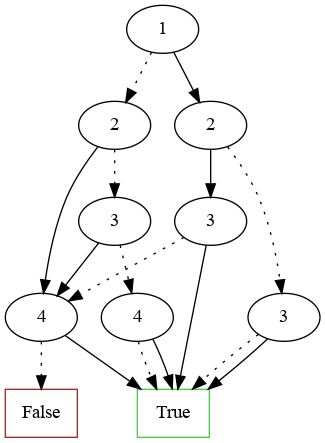
\includegraphics[scale=0.5]{../Images/arbre_compresse_par_arbre.png}
\caption{ZDD construit sur le grand entier [25899],\\ compressé avec \texttt{compressionParArbre}}
\label{fig3}
\end{figure}





\section{Analyse de complexité de notre fonction de compression}

Pour analyser la complexité de l'algorithme, nous compterons cette dernière en nombre de comparaisons \footnote{Que ce soit d'égalité entre deux grands entiers, ou bien dans des structures d'alternatives sur les bits (\texttt{if booléen then [...]} équivaut à comparer le booléen à true et faire le saut correspondant).}. Nous la calculerons d'abord sur la taille de l'arbre. Il sera ensuite possible de passer de la taille de l'arbre à la taille de notre table de vérité par un simple calcul.


Notre fonction de compression prend la forme d'un algorithme de type \textbf{diviser pour mieux régner} : lorsqu'on a un arbre de taille n, on commence par résoudre le problème sur les deux enfants de sa racine, qui sont tout deux de taille majorée par n/2\footnote{C'est le cas avant compression car nous avons un arbre parfait par construction, mais puisqu'on recombine des arbres potentiellement compressés, ils peuvent avoir moins de noeuds}, puis on combine nos deux résultats. Analyser la complexité de notre algorithme nécessite alors d'estimer le coût de cette recombinaison. 

Nous analysons la complexité de la fonction suivante : 

\begin{lstlisting}[basicstyle=\scriptsize]
let compression (arbre : arbre_decision) : arbre_decision = 
    let rec aux (arbre : arbre_decision) (deja_vus : E.ens) : (arbre_decision * E.ens) = 
      let feuilles = liste_feuille arbre in 
      match arbre with
      | Noeud(profond, sag, sad) -> 
          let nouveau_sag, n_deja_vus1 = aux sag deja_vus in
          let nouveau_sad, n_deja_vus2 = aux sad n_deja_vus1 in 
          	(*Regle de compression Z*)
            if (deuxieme_moitie_false feuilles) then (nouveau_sag, n_deja_vus2)
            else 
            (let grand_entier = (composition64 feuilles) in 
              match (E.mem grand_entier n_deja_vus2) with     
              | Some(pointeur) ->
              		(*Regle de compression M*)
              		(pointeur, n_deja_vus2) 
              | None -> 
                	let nouveau_noeud =   (Noeud (profond,nouveau_sag,nouveau_sad))  
                  	in ( nouveau_noeud , (E.insert (grand_entier, nouveau_noeud) n_deja_vus2))    
            )
      | Feuille(booleen) ->  
        (let grand_entier = (composition64 feuilles) in 
          match (E.mem grand_entier deja_vus) with     
          | Some(pointeur) -> 
          	(*Regle de compression M *) 
            (pointeur, deja_vus)                             
          | None -> ( arbre , (E.insert (grand_entier, arbre) deja_vus))             
        )
    in let (g,_) = (aux arbre E.empty) in g

\end{lstlisting}

\bigskip
Dans le cas où notre arbre est sous la forme d'un Nœud : 

\bigskip

\begin{itemize}
\item Deux appels récursifs (\textit{l.6-7}) sur des sous arbres de taille au maximum $\frac{n}{2}$
\item Test sur la liste de feuilles pour faire une sortie anticipée selon la règle Z (\textit{l.9}) 

\textbf{Complexité : $O(log n)$}\footnote{La liste de booléens est de taille log(n), on la parcourt}

\item Calcul du grand entier correspondant au nœud courant (\textit{l.11}) 

\textbf{Complexité : $O(log n)$\footnote{La liste de booléens est de taille log(n), on la parcourt}} 

\item Recherche de ce grand entier dans l'ensemble (\textit{l.12}) 

\textbf{Complexité : $MemE(n)$}, nous la nommons ainsi, il faudra la calculer selon la structure choisie

\begin{itemize}
\item Retourner le nœud trouvé dans l'ensemble s'il y en a un selon la règle de compression M (\textit{l.15}) 

\textbf{Complexité : $O(1)$}

\item Créer un nouveau nœud avec ceux récupérés par les appels récursifs et insérer ce nœud dans l'ensemble sinon (\textit{l.17-18})

\textbf{Complexité : $InsE(n)$}, également à calculer
\end{itemize}

\end{itemize}

\bigskip
Dans le cas où notre arbre est sous la forme d'une Feuille : 
\bigskip

\begin{itemize}
\item Calcul du grand entier correspondant au nœud courant (\textit{l.21})

\textbf{Complexité : $O(log n)$ (idem \textit{l.11}} 

\item Recherche de ce grand entier dans l'ensemble (\textit{l.22}) :

\textbf{Complexité : $MemE(n)$}, (idem \textit{l.12})

\begin{itemize}
\item Retourner le nœud trouvé dans l'ensemble s'il y en a un selon la règle de compression M (\textit{l.25})
\textbf{Complexité : $O(1)$}

\item retourner l'arbre courant et l'insertion de ce dernier dans l'ensemble sinon (\textit{l.26})
\textbf{Complexité : $InsE(n)$}, (idem \textit{l.17-18})

\end{itemize}

\end{itemize}

Notre pire cas est lorsque pour tous nos arbres visités, ils ne sont pas déjà dans l'ensemble, et qu'il faut donc les rajouter\footnote{On pourrait trouver un pire cas plus fin, en réfléchissant sur la combinaison des feuilles étant donné qu'elles ne peuvent prendre que deux valeurs...}.


Étant donné que le pire des cas, pour tout n, est lorsque n n'est pas dans l'arbre, on peut majorer la complexité de notre algorithme par 

$$
T(n) = 2 T(\frac{n}{2}) + 2log(n) + MemE(n) + InsE(n)
$$

Pour approximer cette borne supérieure, nous allons devoirs étudier plus précisément les ordres de grandeur de $MemE(n)$ et $InsE(n)$, qui diffèrent selon l'implémentation.

On rappelle également le théorème maître, qui nous permet de calculer la complexité d'un algorithme type diviser pour mieux régner : 


\begin{tcolorbox}

Soient a $\geq$ 1 et b > 1 deux constantes, soient f une fonction à valeurs dans $\mathbb{R}$ et une fonction de $\mathbb{N}*$ dans $\mathbb{R}^+$ vérifiant pour tout n suffisamment grand l'encadrement suivant : 


\begin{align}
aT(\lfloor\frac{n}{b}\rfloor) + f(n)\leq T(n) \leq aT(\lceil\frac{n}{b}\rceil) + f(n)
\end{align}

Alors T peut être bornée asymptotiquement comme suit : 

\begin{enumerate}
\item Si $f(n) = O(n^{(log_b a)- \epsilon})$ pour une certaine constante $\epsilon > 0$, alors $T (n) = \Theta(n^{log_b a})$. \label{th1}
\item Si $f (n) = \Theta(n^{log_b a})$, alors $T (n) = \Theta(n^{log_b a} log (n))$. \label{th2}
\item Si $f (n) = \Omega(n^{(log_b a)+\epsilon})$ pour une certaine constante $\epsilon > 0$, et si on a pour $c > 1$ $af(\frac{n}{b}) < cf(n)$, alors $T (n) = \Theta(f(n))$. \label{th3}
\end{enumerate}




\end{tcolorbox}


\subsection{Complexité de la fonction \texttt{compresionParListe}}

Dans notre structure de liste : 
\begin{itemize}
\item La complexité d'une insertion est en $O(1)$, étant donné que nous faisons un ajout en tête
\item La complexité d'une recherche est en $O(L)$, où L est la taille de la liste.
\end{itemize}

Or, ici, on fait la supposition d'un pire cas où tous les sous arbres sont différents (notre pire cas théorique), pour un arbre de taille n, L est de l'ordre de grandeur de n. L'insertion est donc en $O(n)$. On peut même la considérer en $\Theta(n)$ dans la mesure où on a fait la supposition que l'arbre n'est pas dans la liste pour avoir le pire cas possible.

On en déduit 

\begin{align*}
T(n) &= 2 T(\frac{n}{2}) + 2log(n) + MemE(n) + InsE(n)\\
&= 2 T(\frac{n}{2}) + O(log n) + O(1) + \Theta (n)\\
&= 2 T(\frac{n}{2}) + \Theta (n)
\end{align*}

Par la règle 2 du théorème maître  \ref{th2}, avec $a = 2$, $b = 2$ et $log_b a = 1$, on obtient 

$$
T(n) = \Theta (n log (n))
$$ 

\medskip

Donc \texttt{compressionParListe (g)} = $O(n log (n))$, où g est un graphe de taille n.


\subsection{Complexité de la fonction \texttt{compresionParArbre}}

Dans notre structure de liste : 
\begin{itemize}
\item La complexité d'une insertion est en $\Theta(L)$, L étant la longueur de la liste de bits, car on va parcourir l'arbre jusqu'à épuiser ses éléments puis insérer l'arbre
\item La complexité d'une recherche est en $O(L)$, L étant la longueur de la liste de bits, car on va parcourir l'arbre jusqu'à épuiser ses éléments puis retourner le nœud courant, ou bien s'arrêter avant si on trouve une feuille.
\end{itemize}

Or, ici, la longueur de la liste de bits correspond au nombre de feuilles de notre arbre, qui est majoré par $log_2 (n)$.

\begin{align*}
T(n) &= 2 T(\frac{n}{2}) + 2log(n) + MemE(n) + InsE(n)\\
&= 2 T(\frac{n}{2}) + O(log n) + O(log(n)) + \Theta (log(n))\\
&= 2 T(\frac{n}{2}) + O(log n)
\end{align*}

Par la règle 1 du théorème maître  \ref{th1}, avec $a = 2$, $b = 2$ et $log_b a = 1$, et le fait que $log(n) = O(n)$\footnote{les logarithmes sont majorés par les fonctions linéaires pour de grandes valeurs} on obtient 

$$
T(n) = \Theta (n ^{log_2 2}) = \Theta(n)
$$ 

\medskip

Donc \texttt{compressionParArbre (g)} = $\theta(n)$, où g est un graphe de taille n.






\section{Étude expérimentale}

\end{document}